%!TEX root = ../username.tex
\chapter{Background} \label{bg}

This section contains the background information necessary to understand the project. % TODO make this more formal

%\section{Mathematical Notation} \label{bg:mathNotation}
% contains notation that may be unfamiliar to readers
% this secion may not be necessary



\section{Musical Terminology and Notation} \label{bg:musicTerminology}
% Musical terms and notation that may be unfamiliar to most readers

% tonic chord tone

\section[Markov Chains]{Markov Chains} \label{bg:markov}

\subsection{Definition} \label{bg:markov:definitions}

A Markov chain is a type of discrete-time stochastic process, which means a Markov chain is a sequence of random variables $\boldsymbol{X} = \{X_{n} | n \in I\}$ for some index set $I$.
Additionally, Markov chains have the special property that they depend only on the immediate past state(s).
That is, for a first-order Markov chain at time $n$, $$P(X_{n} = j \mid X_{0} = i_{0}, \ldots, X_{n - 1} = i_{i - 1}) = P(X_{n} = j \mid X_{n - 1} = i_{n - 1})$$ for a particular possible outcome $j$ of $X_{n}$ \cite{nierhaus_algorithmic_2009}.

This idea can also extend to higher-order Markov chains.
A higher-order Markov process considers more than the single most recent state to determine the next state.
An $n$th order Markov chain uses the previous $n$ states as the input to find the next state.

\subsection{Representations} \label{bg:markov:representations}

We can think of a Markov chain as a directed graph, where each state is a node, each edge is a transition between states, and the probabilities of transitioning between states are represented by the edge weights.
See Figure \ref{fig:markovGraph} for a visual representation of this idea.

\begin{figure}[h]
	\centering
	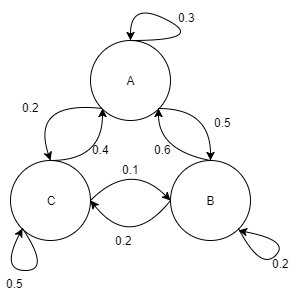
\includegraphics[width=\linewidth]{figures/markovGraph.png} % TODO: Make a better diagram
	\caption{A Markov chain represented as a graph.}
	\label{fig:markovGraph}
\end{figure}

When implementing a Markov chain, however, it is perhaps easier to represent it as an $(n + 1)$-dimensional array, where $n$ is the order of the Markov chain.
We call this $(n + 1)$-dimensional array the transition matrix.
It contains the probabilities of transitioning from one state to another.
See Figure \ref{fig:markovMatrix} for an example of the same Markov chain as in Figure \ref{fig:markovGraph} in matrix form.

\begin{figure}[h]
	\centering
	\begin{tabular}{c | c c c}
		& $A_{1}$ & $B_{1}$ & $C_{1}$\\
		\hline
		$A_{0}$ & $0.3$ & $0.5$ & $0.2$\\
		$B_{0}$ & $0.6$ & $0.2$ & $0.2$\\
		$C_{0}$ & $0.4$ & $0.1$ & $0.5$
	\end{tabular}
	\caption{A Markov chain represented as a transition matrix.}
	\label{fig:markovMatrix}
\end{figure}

\subsection{Limitations} \label{bg:markov:limitations}

A major limitation of Markov chains is their inability to generate truly novel output.
In order for some state to appear, a transition to that state from the previous state must appear in the source material.
That is, no truly novel transitions may appear; all transitions that appear in the output of the Markov chain must have appeared somewhere before.
Additionally, lower-order chains may produce nonsensical output, whereas a chain of sufficiently high order will exactly copy the source material.
Another limitation is that the process may get stuck in a ``local loop''.
This may happen when the chain proceeds to a state which only transitions to itself, or transitions to a set of states that only transition to each other.

%\section{Neural Networks} \label{bg:nn}
% maybe? would give brief crash course of NNs


\section{Genetic Algorithms} \label{bg:ga}
% a beief crach course on GAs
%\subsection{Definition}

In general, a genetic algorithm takes an initial population and produces a new set of individuals to become the initial population of the next generation.
This new set is produced by performing various operations on the initial population, then using a fitness function to choose the best performing individuals.
Common operation on the initial population include combining individuals in different ways, similar to how genetic information from two parents is combined into a child, and introducing mutations. % TODO go more in-depth here
That is, making small random changes to individuals in the population.

To choose the new initial population, a fitness function is defined which measures how close an individual is to the desired output.
If some individuals reach a certain level fitness, they are the output of the genetic algorithm.
Otherwise, the best performing individuals become the initial population of the next generation.
This process continues until some individuals perform well enough.
